%____________________________________________________________________________||
\section{Variation of yields in the sideband and control regions under systematic variation}
\label{app:prop-shift-syst}
This section includes the propotional shift of the yields in the sideband and control regions
under different systematic variations. This is defined by the ratio of the yields predicted after
the variation of the systematic source to the nominal yield. The systematic shift predicted for the
\mj, \mmj and \gj control regions are shown in 
Fig.\ref{fig:cr-shift} and the variations for the respective sideband 
regions are shown in Fig.\ref{fig:sideband-shift}. 
The uncertainties shown are representative of the statistical
power of the sample. The ratio between the shift for sideband and control 
regions is then used to produce Figs.\ref{fig:pho-bias-sideband}-\ref{fig:mumu-bias-sideband}. 

\begin{figure}[!h]
  \centering
  \subfigure[\gj control region]{
  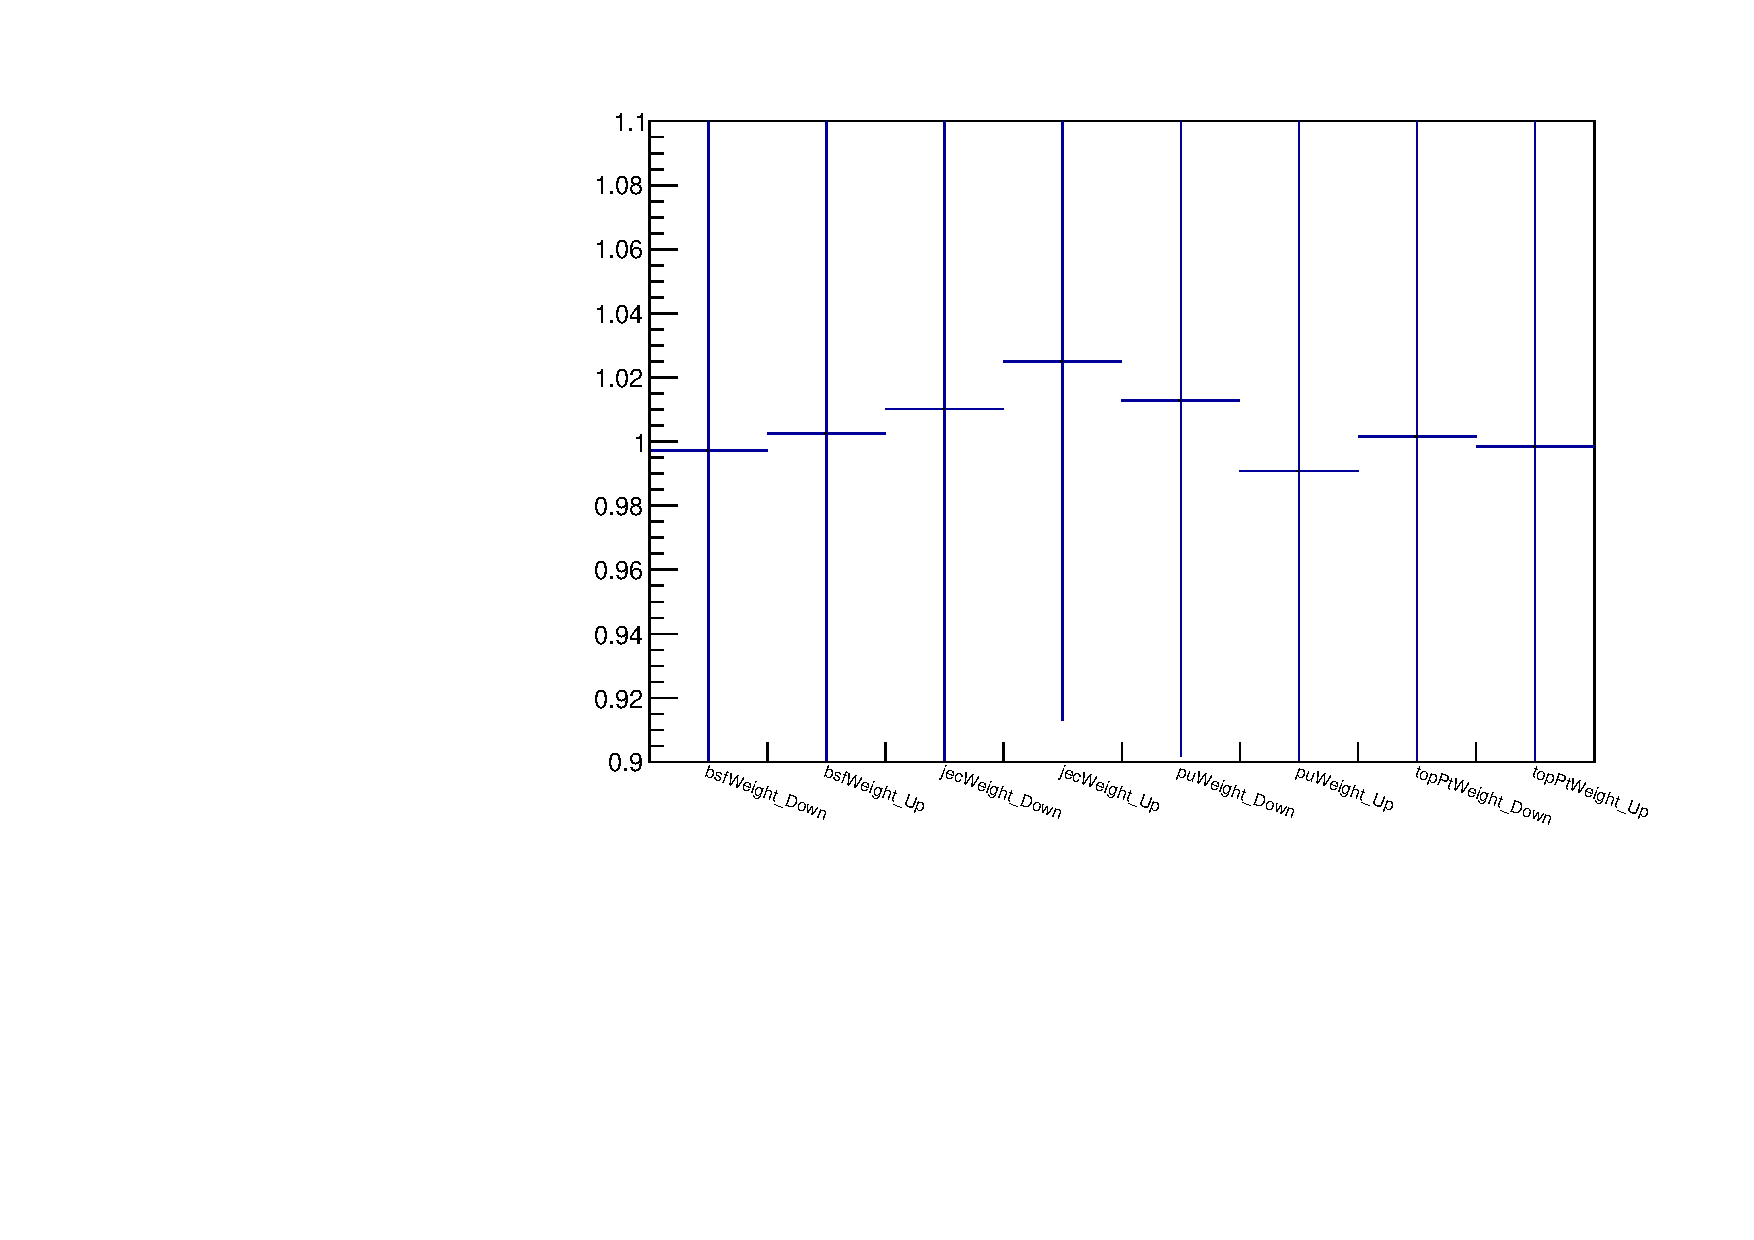
\includegraphics[width=0.45\textwidth]{figures/sideband_fit/summary_MhtSB_SinglePhotonSB.pdf}
  }
  \subfigure[\mj control region]{
  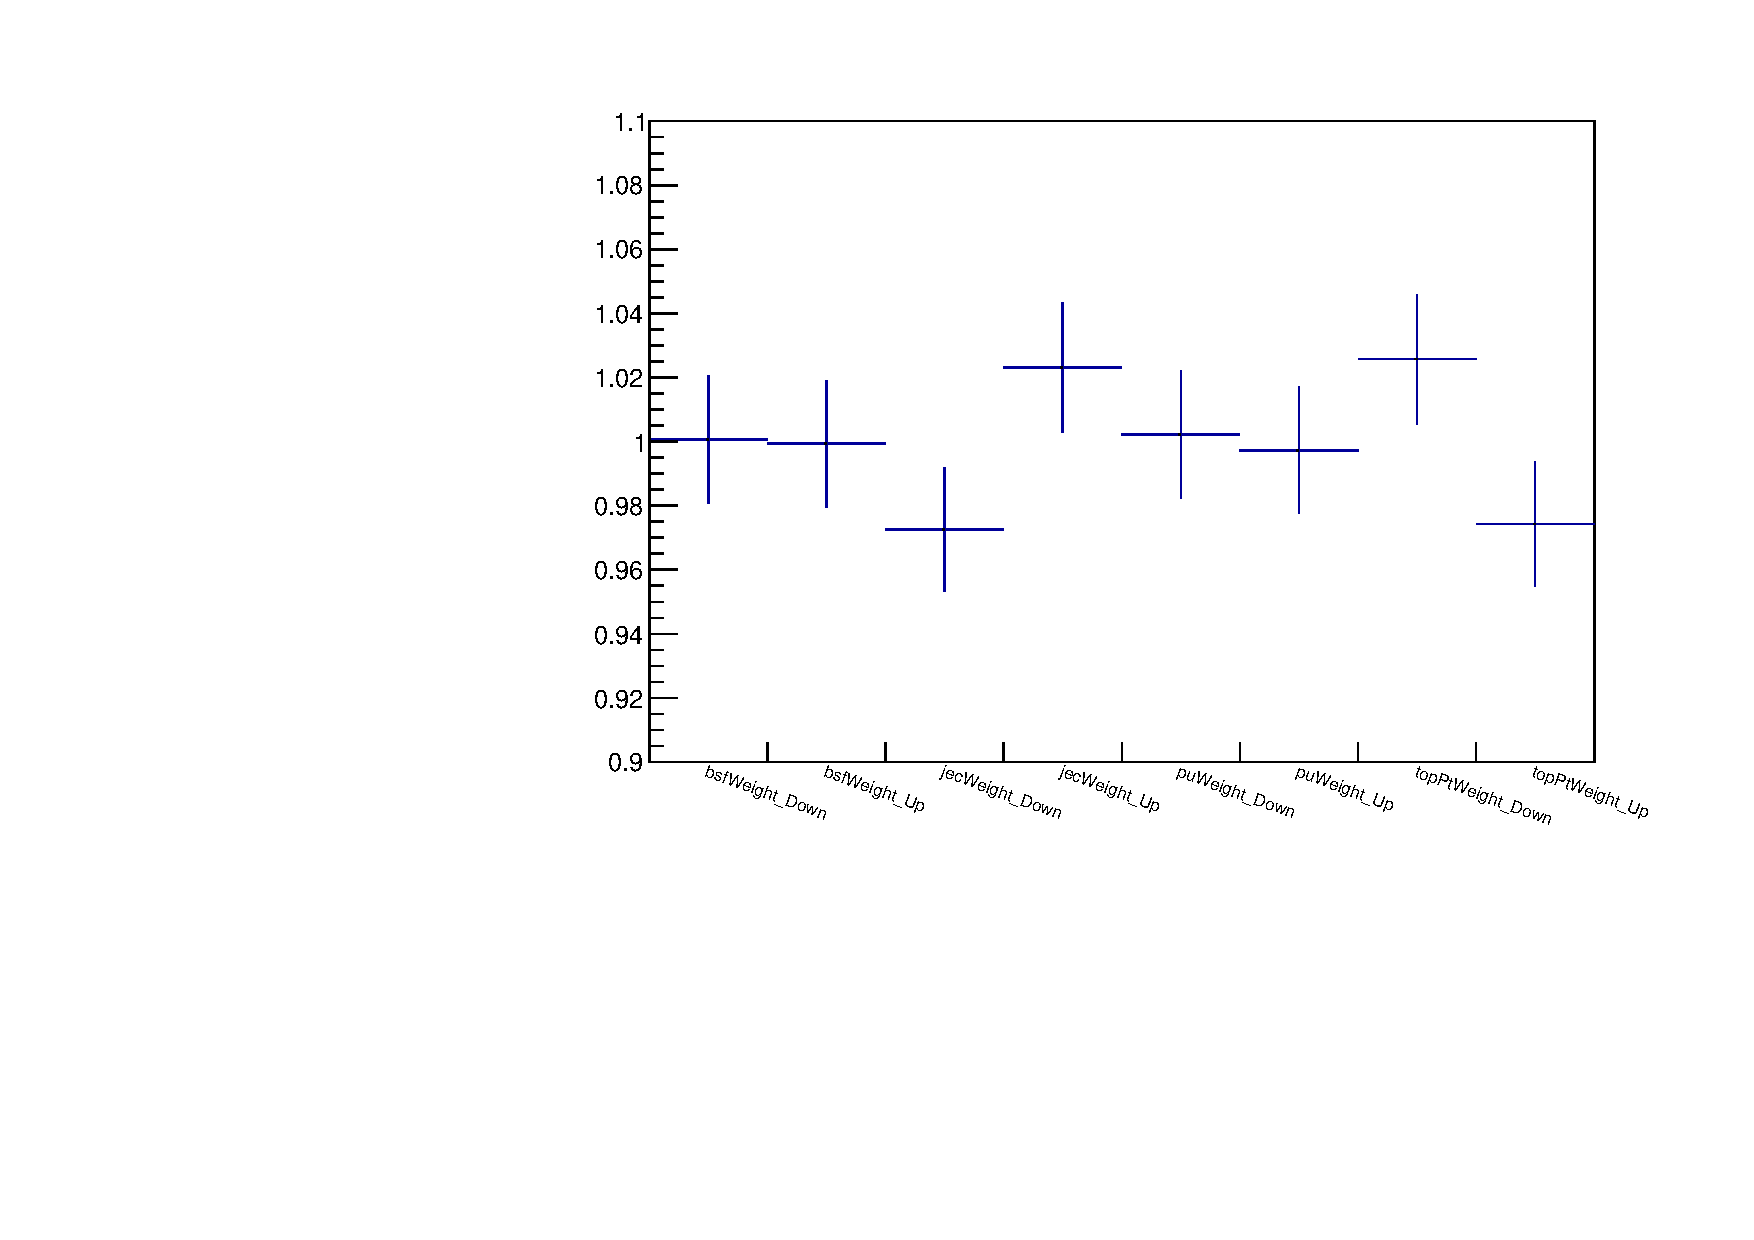
\includegraphics[width=0.45\textwidth]{figures/sideband_fit/summary_MhtSB_SingleMuSB.pdf}
  }\\
  \subfigure[\mmj control region]{
  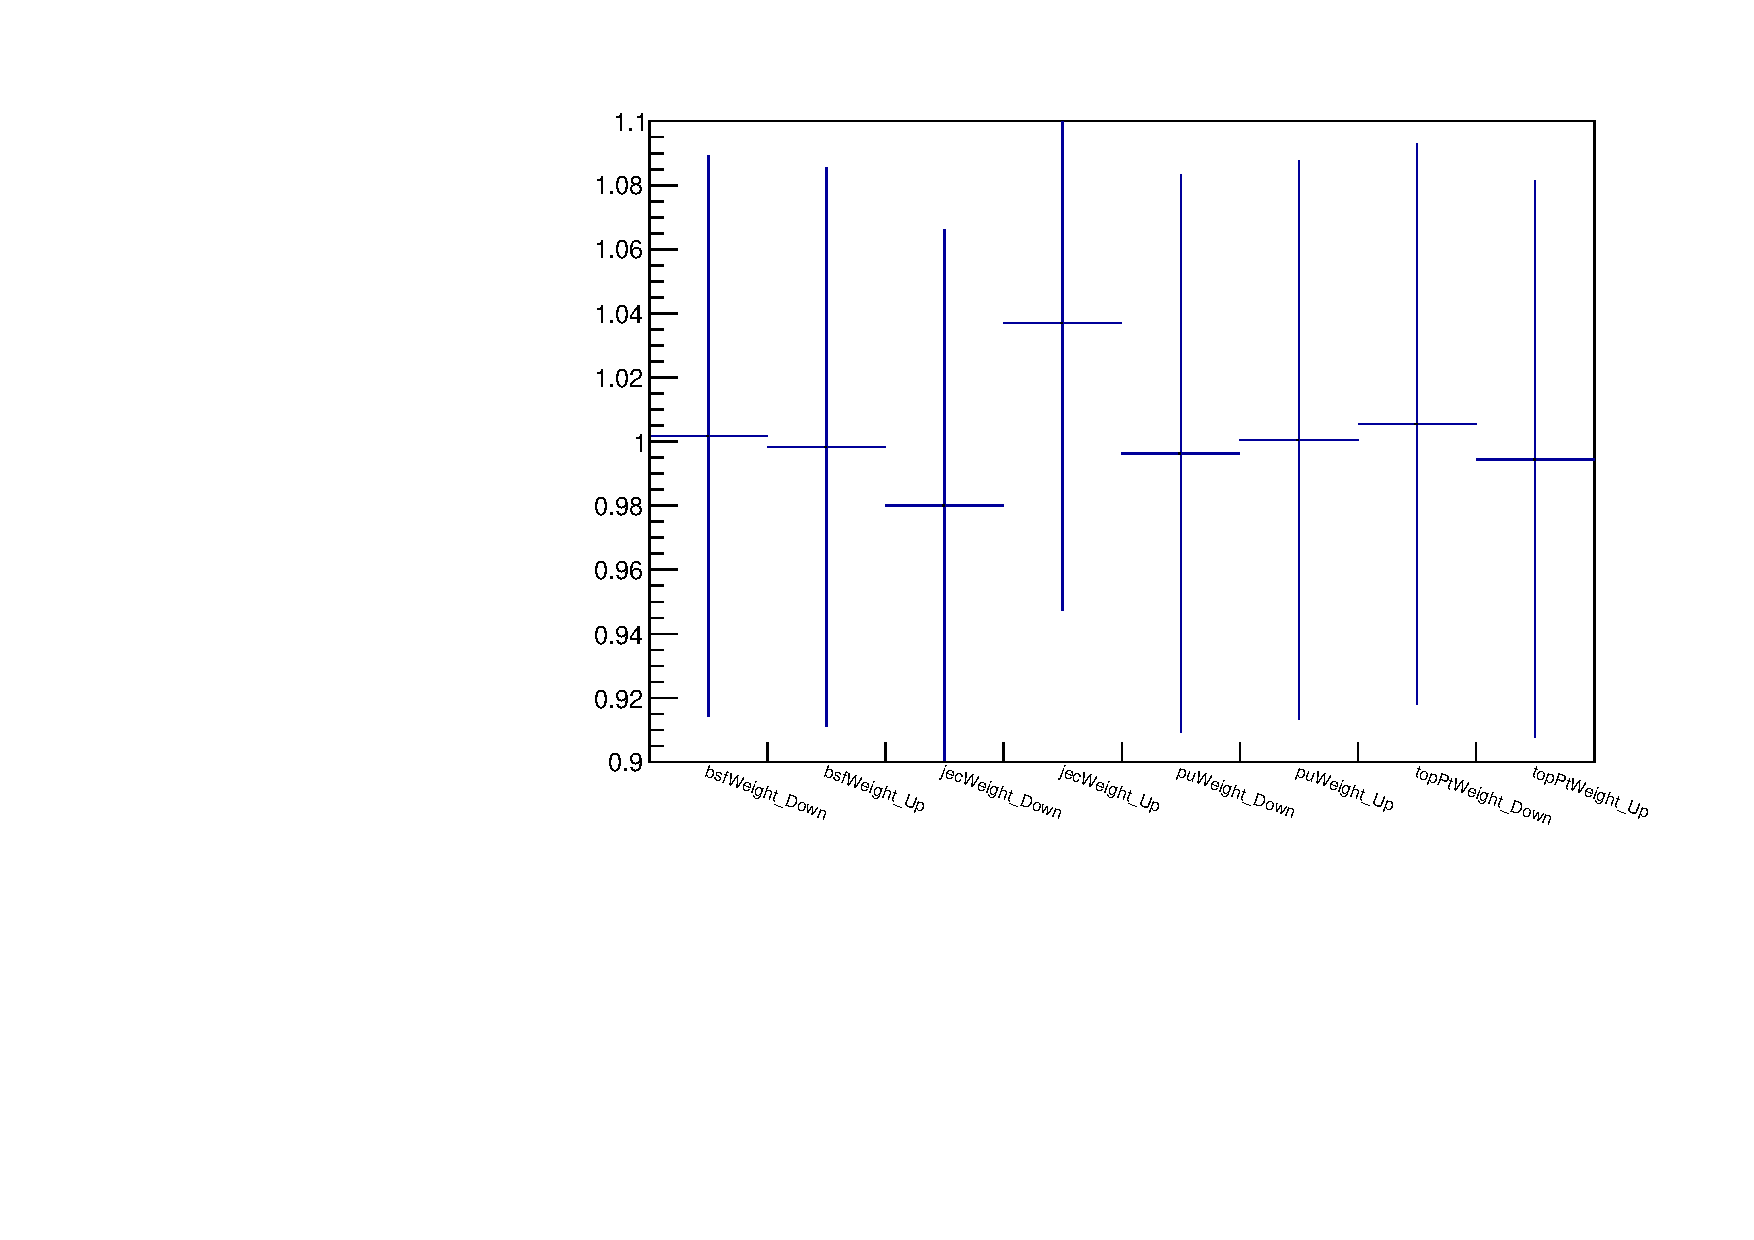
\includegraphics[width=0.45\textwidth]{figures/sideband_fit/summary_MhtSB_DoubleMuSB.pdf}
  }
  \caption{The proportional shift in prediction in the sideband regions under various known systematics.
  The uncertainties shown are representative of the statistical power of the sample}

  \label{fig:sideband-shift}
\end{figure}

\begin{figure}[!h]
  \centering
  \subfigure[\gj control region]{
  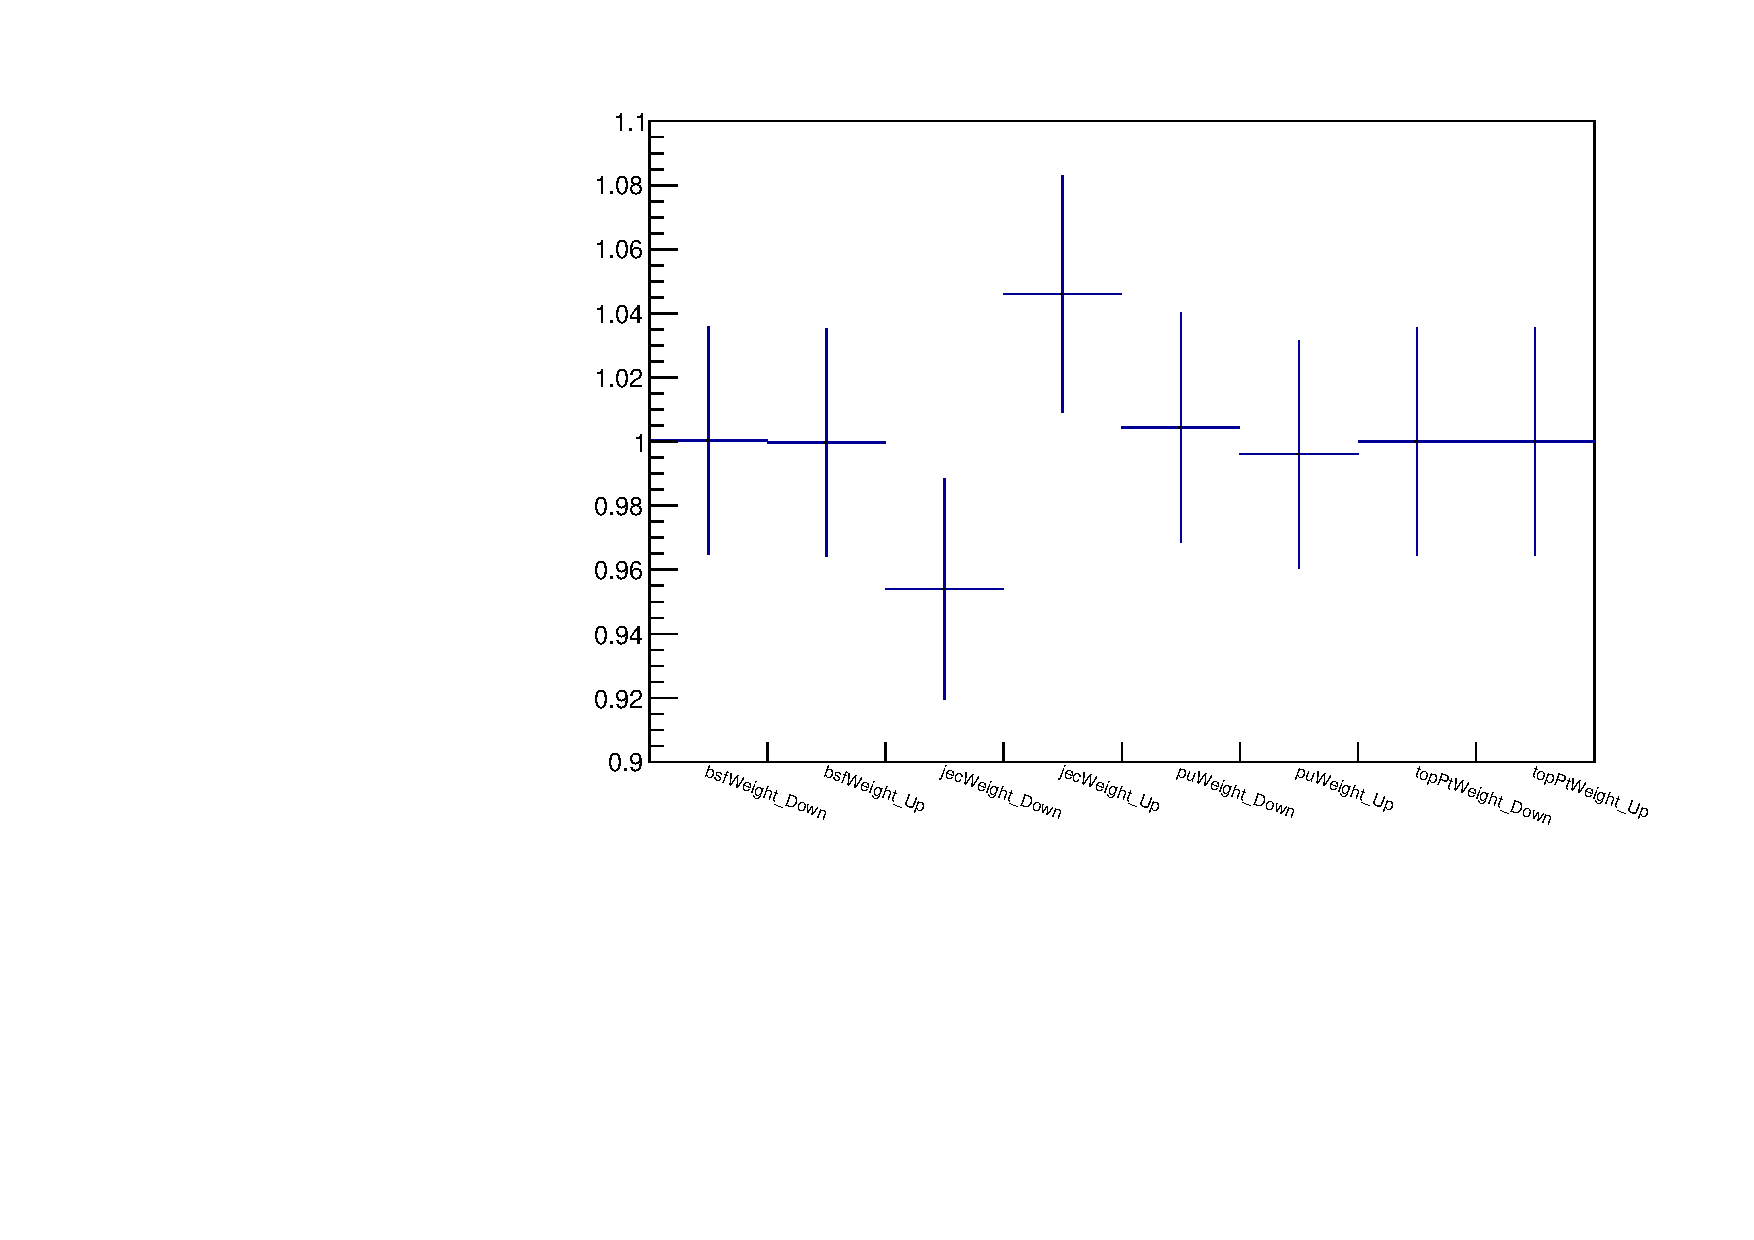
\includegraphics[width=0.45\textwidth]{figures/sideband_fit/summary_MhtSB_SinglePhotonCR.pdf}
  }
  \subfigure[\mj control region]{
  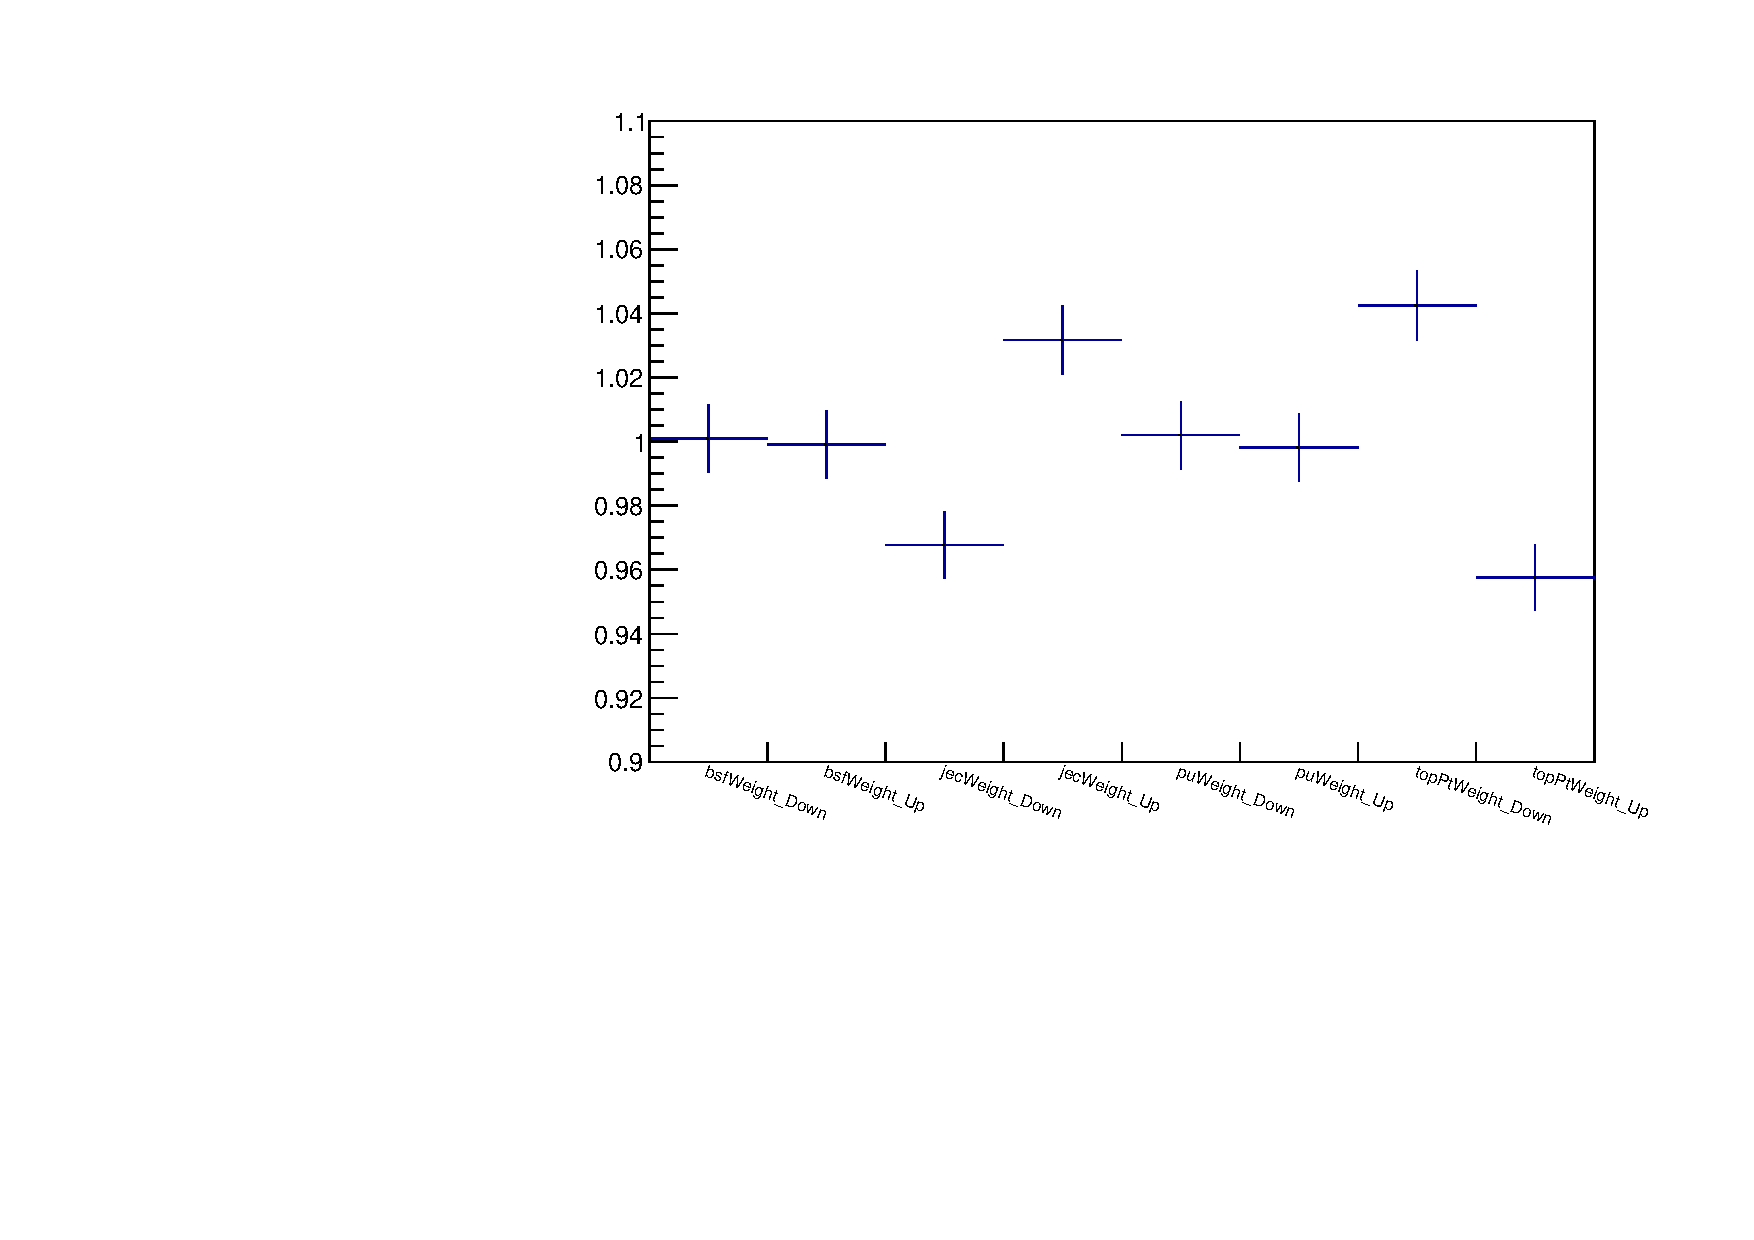
\includegraphics[width=0.45\textwidth]{figures/sideband_fit/summary_MhtSB_SingleMuCR.pdf}
  }\\
  \subfigure[\mmj control region]{
  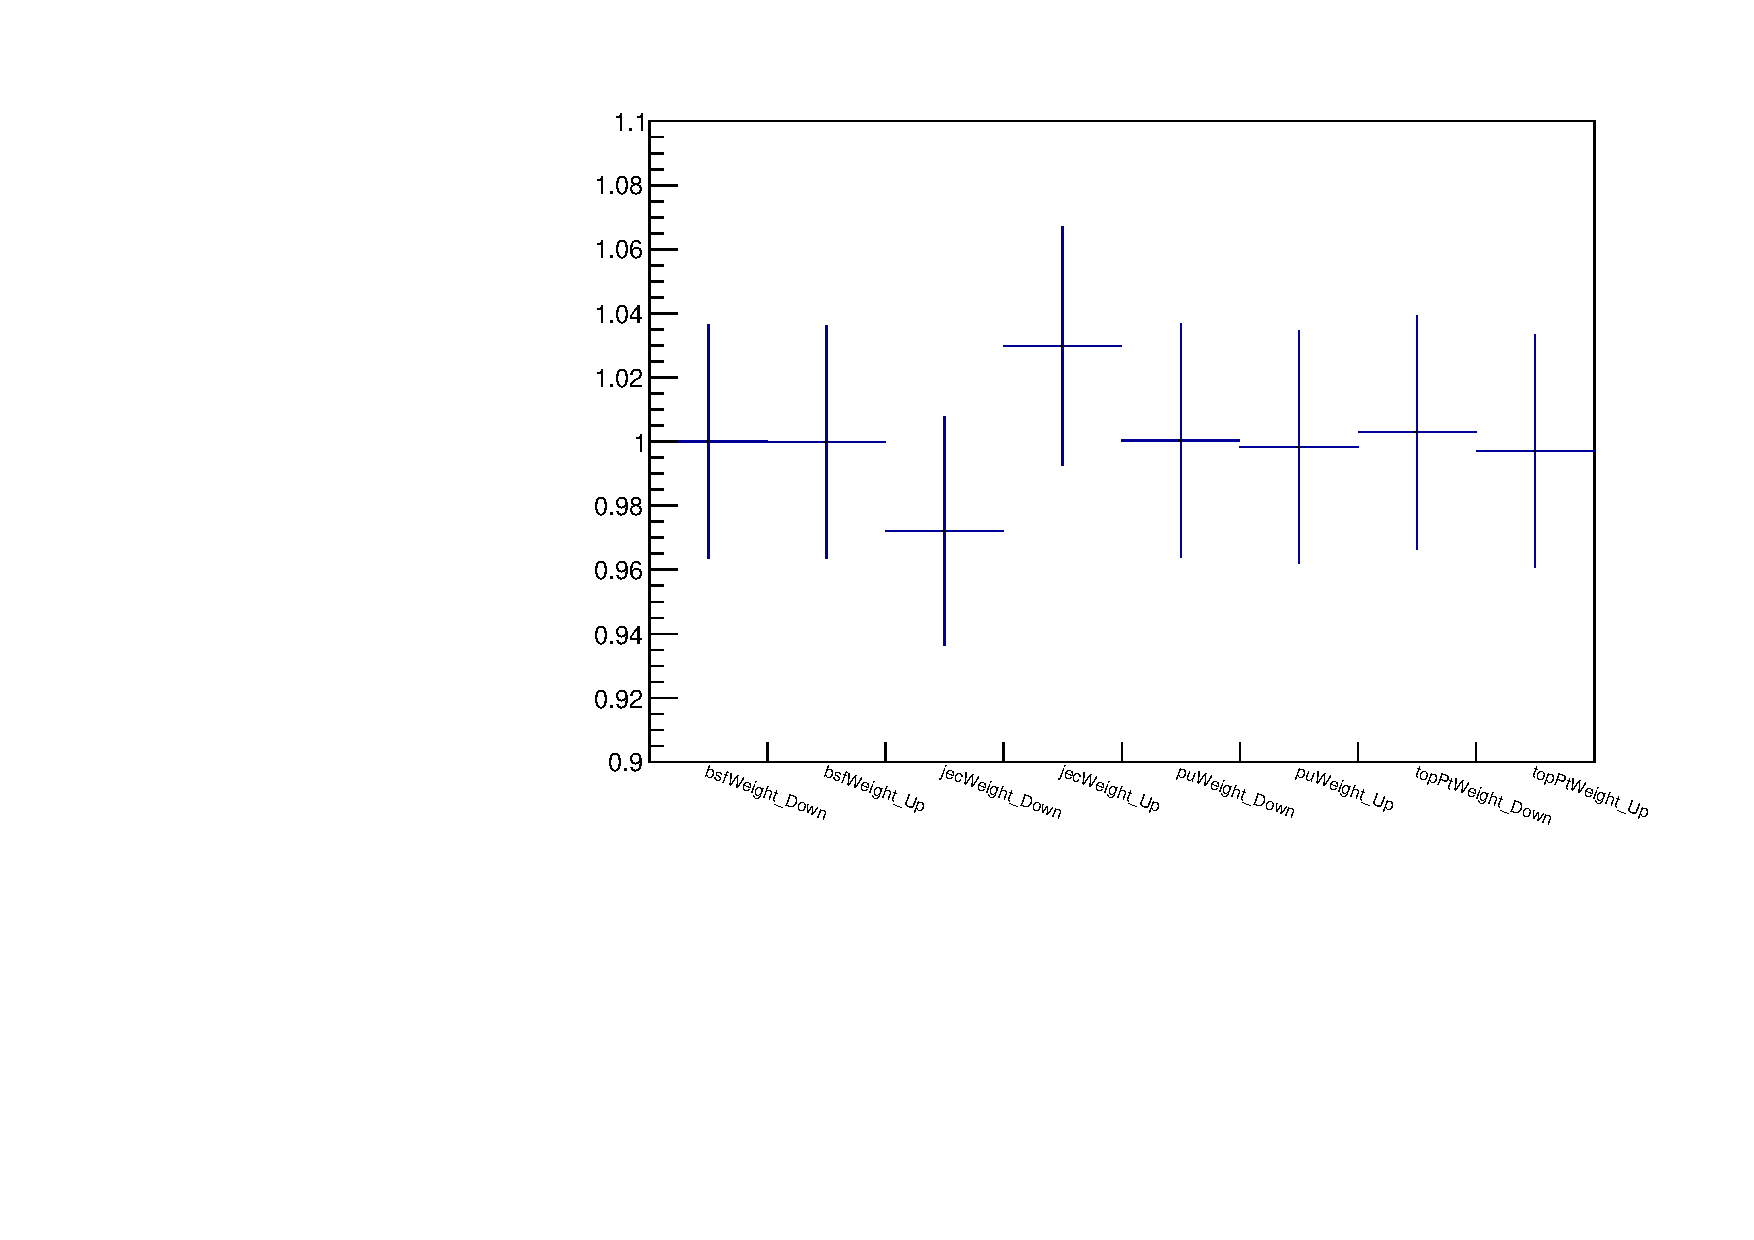
\includegraphics[width=0.45\textwidth]{figures/sideband_fit/summary_MhtSB_DoubleMuCR.pdf}
  }
  \caption{The proportional shift in prediction in the control regions under various known systematics. 
  The uncertainties shown are representative of the statistical power of the sample}
  \label{fig:cr-shift}
\end{figure}

